% This is samplepaper.tex, a sample chapter demonstrating the
% LLNCS macro package for Springer Computer Science proceedings;
% Version 2.21 of 2022/01/12
%
\documentclass[runningheads]{llncs}
%
\usepackage[T1]{fontenc}
% T1 fonts will be used to generate the final print and online PDFs,
% so please use T1 fonts in your manuscript whenever possible.
% Other font encondings may result in incorrect characters.
%
\usepackage{graphicx}
\usepackage{tikz}
% Used for displaying a sample figure. If possible, figure files should
% be included in EPS format.
%
\usepackage{hyperref}
% If you use the hyperref package, please uncomment the following two lines
% to display URLs in blue roman font according to Springer's eBook style:
\usepackage{color}
\renewcommand\UrlFont{\color{blue}\rmfamily}
\urlstyle{rm}

\usepackage{amssymb}
\newcommand{\QQ}{\mathbb Q}
\newcommand{\ZZ}{\mathbb Z}

%
\begin{document}
%
\title{A Macaulay2-Lean interface for proofs in Lean}
%
%\titlerunning{Abbreviated paper title}
% If the paper title is too long for the running head, you can set
% an abbreviated paper title here
%
\author{
  Matthew Ballard\inst{1}\orcidID{0000-0001-5819-0159} \and
  Anton Leykin\inst{2}\orcidID{0000-0002-9216-3514} \and
  Michael E. Stillman\inst{3}\orcidID{0000-0003-0078-3116} \and
  Damiano Testa\inst{4}\orcidID{0009-0004-5949-6861} \and
  Douglas A. Torrance\inst{5}\orcidID{0000-0003-3999-4973} \and
  Jay Yang\inst{6}\orcidID{0000-0001-8366-423X}
  }
%
\authorrunning{M. Ballard et al.}
% First names are abbreviated in the running head.
% If there are more than two authors, 'et al.' is used.
%
\institute{University of South Carolina, Columbia SC 29208, USA \email{ballard@math.sc.edu} \and
  Georgia Institute of Technology, Atlanta GA 30332, USA \email{leykin@math.gatech.edu} \and
  Cornell University, Ithaca NY 14850, USA \email{mes15@cornell.edu}\and
  University of Warwick, Coventry CV4 7AL, UK \email{D.Testa@warwick.ac.uk} \and
  Piedmont University, Demorest GA 30535 \email{dtorrance@piedmont.edu} \and
  Vanderbilt University, Nashville TN 37235 \email{jay.k.yang@vanderbilt.edu}}
%
\maketitle              % typeset the header of the contributioln
%
\begin{abstract}

  Our project aims to build tools that ease the use of Macaulay2 and potentially other computer algebra systems with Lean.
Our current work focuses on using Macaulay2 to prove statements over commutative rings by using Macaulay2 to construct certificates. This includes in particular work with ideal membership and Groebner bases.
This extend abstract discuss our approach and strategy along with current progress and future goals.
%This is work with Matthew Ballard, Anton Leykin, Damiano Testa, and Doug Torrance as part of the ``Bridging Proof and Computation'' project sponsered by Renaissance Philanthropy.

\keywords{First keyword  \and Second keyword \and Another keyword.}
\end{abstract}
%
%
%

\section{Introduction}

\cite{lean}
\cite{M2}

\section{Design}

As a general matter of design, an interface with a computer algebra system intended to prove statements in Lean must contain the following steps described in Figure\ref{fig:steps}:
\begin{enumerate}
\item Start with a proposition and hypotheses for a statement provable using the CAS
\item Extract a computational problem from the proposition and hypotheses.
\item Send the data to the CAS, including serialization and deserialization by Lean and Macaualy2 respectively.
\item Solve the problem using the CAS, Resulting in a solution and a certificate in the form of some mathematical data
\item Send the solution and the certificate to Lean, including again serialization and deserialization.
\item Convert the solution and certificate to a proof of the original proposition.
\end{enumerate}

\begin{figure}
  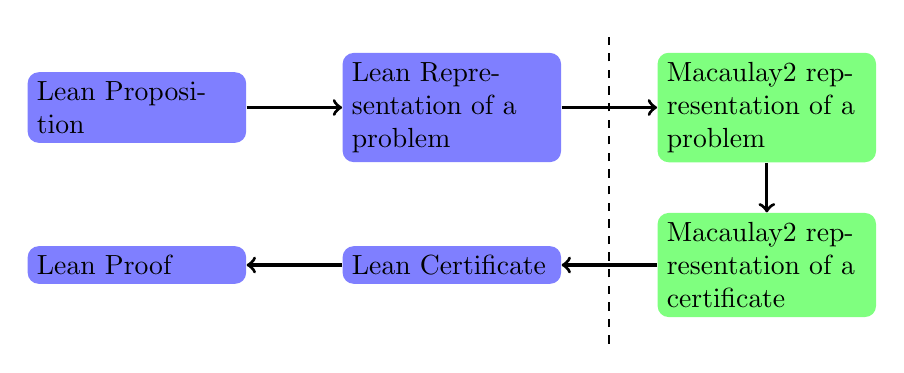
\begin{tikzpicture}
    \begin{scope}[fill opacity = 0.5, text opacity = 1,rounded corners]
      \node[fill = blue,text width = 1in] (prop) at (0,0) {Lean Proposition};
      \node[fill = blue,text width = 1in] (lean-prob) at (4,0) {Lean Representation of a problem};
      \node[fill = green,text width = 1in] (m2-prob) at (8,0) {Macaulay2 representation of a problem};
      \node[fill = green,text width = 1in] (m2-sol) at (8,-2) {Macaulay2 representation of a certificate};
      \node[fill = blue,text width = 1in] (lean-sol) at (4,-2) {Lean Certificate};
      \node[fill = blue,text width = 1in] (lean-proof) at (0,-2) {Lean Proof};
    \end{scope}
    \draw[->,very thick] (prop) -- (lean-prob);
    \draw[->,very thick] (lean-prob) -- (m2-prob);
    \draw[->,very thick] (m2-prob) -- (m2-sol);
    \draw[->,very thick] (m2-sol) -- (lean-sol);
    \draw[->,very thick] (lean-sol) -- (lean-proof);

    \draw[dashed, thick] (6,-3) -- (6,1);
  \end{tikzpicture}
  \caption{The general steps by which a Lean proposition can be proved using a certificate from Macaulay2}
  \label{fig:steps}
\end{figure}


We emphasize here that the problem is different than the proposition, and the certificate is distinct from the proof. The problem consists of the mathematical data needed to construct the certificate and the certificate consists of the mathematical data needed to construct the proof. This separation of the problem and the proposition along with the certificate and the proof is important, because are instances where two different classes of proposition may be solvable using the same underlying problem and certificate. This decouples the proof goal from the computational goal.

For each potential class of problem to be solved using a computer algebra system, the exact details of the the content of both the problem and the certificate need to be defined and potentially tailored to the relevant computer algebra system. However, there is a common task of serializing and deserializing mathematical expressions. While here again the exact format needs to be tailored to the computer algebra system in question, we discuss in Section~\ref{} our approach. Moreover, while it is not within the scope of our current work, a more general system may define mechanisms for the discovery of problems solvable by computer algebra systems.

\subsection*{The Ideal Membership Tactic}
This basic framework is the how the two primary tactics we currently implement, \verb|m2idealmem| and \verb|m2remainder|, work.

Focusing specifically on \verb|m2idealmem|, it is designed to solve the vanishing of a polynomial subject to the vanishing of other polynomials. For example, the code will correspond to the following parts
\begin{verbatim}
example {x y : Rat} (f : 2*x= 0) (g : 3*y = 0) : (x + y)^4 = 0 := by
  m2idealmem [f,g]
\end{verbatim}


\begin{figure}
  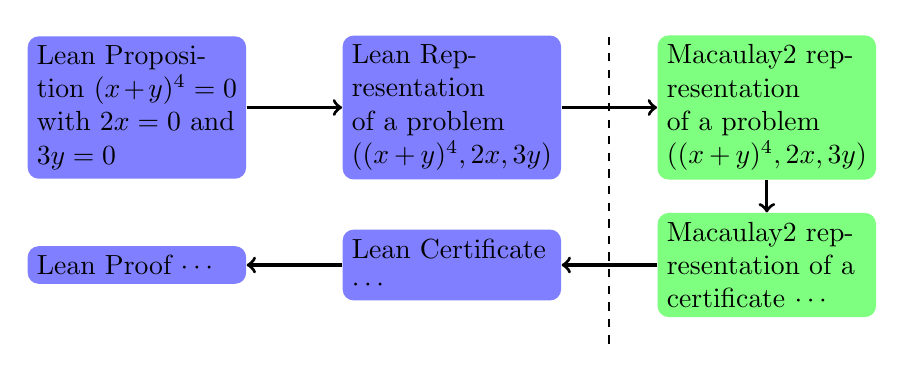
\begin{tikzpicture}
    \begin{scope}[fill opacity = 0.5, text opacity = 1,rounded corners]
      \node[fill = blue,text width = 1in] (prop) at (0,0) {Lean Proposition $(x+y)^4=0$ with $2x=0$ and $3y=0$};
      \node[fill = blue,text width = 1in] (lean-prob) at (4,0) {Lean Representation of a problem $((x+y)^4,2x,3y)$};
      \node[fill = green,text width = 1in] (m2-prob) at (8,0) {Macaulay2 representation of a problem $((x+y)^4,2x,3y)$};
      \node[fill = green,text width = 1in] (m2-sol) at (8,-2) {Macaulay2 representation of a certificate $\cdots$};
      \node[fill = blue,text width = 1in] (lean-sol) at (4,-2) {Lean Certificate $\cdots$};
      \node[fill = blue,text width = 1in] (lean-proof) at (0,-2) {Lean Proof $\cdots$};
    \end{scope}
    \draw[->,very thick] (prop) -- (lean-prob);
    \draw[->,very thick] (lean-prob) -- (m2-prob);
    \draw[->,very thick] (m2-prob) -- (m2-sol);
    \draw[->,very thick] (m2-sol) -- (lean-sol);
    \draw[->,very thick] (lean-sol) -- (lean-proof);

    \draw[dashed, thick] (6,-3) -- (6,1);
  \end{tikzpicture}
  \caption{The specific data in reference to Figure~\ref{fig:steps} in the case of one potential ideal membership problem}
  \label{fig:steps-example}
\end{figure}


NOTE: we should have an example that illustrates the subtleties with representations of polynomials and the sizes of the terms that can be involved even for seemingly ``small'' problems. Possibly cite the big benchmark example and give some numbers on how big it is.

Then to show vanishing, it suffices to show that $(x+y)^4$ is in the ideal $\langle 2x, 3y\rangle\subseteq \mathbb{Q}[x,y]$.

We send the expanded polynomial $f(x,y) = x^4+4x^3y+6x^2y^2+4xy^3+y^4$ to Macaulay2 along with the ideal generators $2x$ and $3y$. Then Macaualy2 will compute polynoials $q_1,q_2,r\in \mathbb{Q}[x,y]$ such that $q_1(x,y)\cdot 2x + q_2(x,y)\cdot 3y=f(x,y) = r(x,y)$.
The polynomials $q_1$ and $q_2$ are not unique, and so a topic of some relevance is choosing optimal polynomials. Macaulay2 may not return polynomials that are computationally optimal. In this case the polynoials returned are $q_1(x,y) = \cdots$, and $q_2(x,y)= \cdots$. TODO FILL IN

In the case of ideal membership, if the equality is expected, we should get $r=0$. Note that failure of ideal membership does not provide a disproof of the equality statement at hand.

After this computation, we effectively have two polynomial equalities to prove.

\begin{enumerate}
\item We want to show that subject to the constraints $2x=0$ and $3y=0$, that $q_1\cdot 2x + q_2\cdot 3y = 0$. This is proved by simply rewriting the expression using the equalities provided, and we do this directly.
\item We want to show that the polynomials $q_1\cdot 2x + q_2 \cdot 3y =  x^4+4x^3y+6x^2y^2+4xy^3+y^4$. In theory this is simply a repeated application of the distributive, commutative, and associative laws. However, these expressions can be quite large, and so a significant difficulty which we do not yet address is the efficient proof of this equality.
  For now we have an optional step to use the grind tactic to prove this polynomial equality, or we leave it to the user of the tactic to prove the equality, via whatever methods are relevant to the specific problem. Giving an efficient implementation of this step is a key step in our future directions \ref{}. 
\end{enumerate}

\subsection*{Universalization to $\mathbb{Z}$}

There is one final feature of our current work of note.
Not every ring has an easy representation that allows serialization to Macaulay2. However, even over general rings, many problems are rephrasable in terms of problems for integers and many polynomials have coefficients over the integers. As such, instead of providing an error when encountering an unknown ring, we first attempt to rephrase the question over the integers.

\section{Implementation}

\subsection*{Communication}

Due to its simplicity and ubiquity, it was decided that JSON (JavaScript Object Notation) would be used to facilitate communication between Macaulay2 and Lean.  In particular, the top-level communication is handled by the JSON-RPC protocol \cite{jsonrpc} and the mathematical objects are serialized using the MRDI file format \cite{mrdi}.

The ``RPC'' in JSON-RPC stands for \textit{remote procedure call}.  It is a protocol that defines a set of JSON objects for clients to make requests and servers to send responses.  It is the foundation of the Language Server Protocol \cite{lsp} used by a wide variety of editors and which is fundamental to the user experience in Lean.  Since both Lean and Macaulay2 already support JSON-RPC, it was a natural choice upon which to build the interface.

The MRDI file format is used for serializing mathematical objects in the OSCAR computer algebra system \cite{OSCAR-Book,OSCAR}, but it was designed with the idea that it could be used for the same purpose in other systems.  Each MRDI file contains a single JSON object with at least one key, \texttt{\_type}, for specifying the particular type of the object.  Additionally, it may have a \texttt{\_ns} key for specifying the namespace (such as the particular computer algebra system), a \texttt{data} key for information about the object.  Some of the values under the \texttt{\_type} and \texttt{data} keys may contain \textit{universally unique identifiers} (or UUID's) for additional objects, and further information about these objects is stored under the \texttt{\_refs} key.

Consider, for example, the polynomial $3x^2 + \frac{1}{2}\in\QQ[x]$.  We store this as $3y_0^2 + y_1\in\ZZ[y_0,y_1]$ together with the map $y_1\mapsto\frac{1}{2}$.  See the example below.

\begin{verbatim}
{"_type": {"params": "Rat", "name": "ConcretePoly"},
 "data": {"poly": "a8ea4eb2-4393-45b0-ba9a-0c91716a55d3",
          "coefficients": [["1", ["1", "2"]]]},
 "_ns": {"Lean": ["https://github.com/leanprover/lean4", "4.26.0-rc1"]},
 "_refs": {"a8ea4eb2-4393-45b0-ba9a-0c91716a55d3":
            {"_type": "LeanGrindCommRingPoly",
             "data": [["3", [["0", "2"]]], ["1", [["1", "1"]]]]}}}
\end{verbatim}

Putting these pieces together, if we want Lean to delegate a computation to Macaulay2, then we may serialize any associated mathematical objects using MRDI, pass these as arguments to an appropriate method and send the corresponding JSON-RPC request to a server running in Macaulay2, de-serialize the mathematical objects in Macaulay2, run the requested computation, serialize any mathematical objects produced by this computation, pass the result in a JSON-RPC response back to Lean, and finally de-serialize the result in Lean.

\subsection*{Polynomial Representation}

For convenience, our current efforts reuse significant parts of the infrastructure of the \verb|grind| tactic. As such, polynomials are represented using the \verb|Lean.Grind.CommRing.Poly| type.
However, as this type models polynomials with integer coefficients, there are significant constraints to this 

\section{Future Goals}

As this is a project in progress, there is significant work that still needs to be done.

\subsection*{Other Computations}

TODO

\subsection*{Stored Computations}
One goal is to make it easier to separate the calls to Macaualy2 and the actual proof in Lean. While for interactive and smaller proofs, the disadvantages is the requirement that a copy of Macaulay2 has to be installed whenever the the proof is to be checked. For this reason, a future goal is to add the ability to store the result of a tactic call to a file as to allow the computational step to run once and be exported to be used.

There are two key advantages to such a format
\begin{enumerate}
\item Reproducibility: If the computation is done once and exported
\item Scalability: (I don't actually like phrasing it as scallability, but the point is correct) For larger computations, it is highly plausible that the computation may require resources, in the form of time or memory, beyond what is reasonable for the computer running the lean code. In such circumstances, to be able to cleanly export the problem is useful for separating the computation and the proof.
\end{enumerate}

Here the use of the MRDI format makes it easier to achive this objective as MRDI is a format already desgined for storage and export/import \cite{}.

\subsection*{Polynomial Format}

While the current polynomial format maximizes reuse of grind related code, it is not clear that it is optimal for our purposes. Other possibilities include ....

The two major issues that need to be solved are the scale of the polynomials and the ease of communication with Macaulay2.

Even when the problems are relatively small, either the Groebner basis or the coefficients used can be quite large. As an example of the potential scale of computations, The ideal membership problem for the question from ... is esentially immediate in Macaulay2. However equality of the resulting expressions is difficult to prove in lean using current tools due to the size of the expressions involved. Naive attempts at direct expansion using distributive, associative, and commutative laws tend to create very large proof terms.


\begin{credits}
  \subsubsection{\ackname} The work in this paper was funded by the Renaissance Philanthropy AI for Math Grant ``Bridging Proof and Computation''.

  %A bold run-in heading in small font size at the end of the paper is
%used for general acknowledgments, for example: This study was funded
%by X (grant number Y).

\subsubsection{\discintname}
The authors have no competing interests to declare that are
relevant to the content of this article.
\end{credits}
%
% ---- Bibliography ----
%
% BibTeX users should specify bibliography style 'splncs04'.
% References will then be sorted and formatted in the correct style.
%
\bibliographystyle{splncs04}
\bibliography{mybibliography}
\end{document}
